% PROSZĘ KOMPILOWAĆ TEN DOKUMENT ZA POMOCĄ SILNIKA XELATEX
% W PRZECIWNYM RAZIE NALEŻY USUNĄĆ PAKIET fontspec ORAZ USTAWIENIA FONTU
% Z PLIKU styles/prez_wmini_pl.sty (PIERWSZE TRZY LINIJKI)
% W PRZYPADKU BRAKU FONTU Adagio Slab NALEŻY ZGŁOSIĆ SIĘ DO BIP PW O JEGO UDOSTĘPNIENIE,
% ZAŁADOWAĆ INNY KRÓJ CZCIONKI LUB ZAKOMENTOWAĆ/USUNĄĆ USTAWIENIA FONTU

\documentclass[aspectratio=169]{beamer}

\usepackage{styles/prez_wmini_pl}
\usepackage{booktabs}
\setbeamertemplate{section in toc}[sections numbered]
\setbeamertemplate{subsection in toc}[subsections numbered]
\usepackage{times}
\usepackage{amsmath}
\usepackage{bm}

\usefonttheme[onlymath]{serif}

\definecolor{quotationcolour}{HTML}{F0F0F0}
\definecolor{quotationmarkcolour}{HTML}{1F3F81}

% Double-line for start and end of epigraph.
\newcommand{\epiline}{\hrule \vskip -.2em \hrule}
% Massively humongous opening quotation mark.
\newcommand{\hugequote}{%
  \fontsize{42}{48}\selectfont \color{quotationmarkcolour} \textbf{``}
  \vskip -.5em
}

% Beautify quotations.
\newcommand{\epigraph}[2]{%
  \bigskip
  \begin{center}
  \colorbox{quotationcolour}{%
    \parbox{.80\textwidth}{%
    \epiline \vskip 1em {\hugequote} \vskip -.5em
    \parindent 2.2em
    #1\vspace{-.25cm}\begin{flushright}\textsc{#2}\end{flushright}
    \epiline
    }
  }
  \end{center}
  \bigskip
}

\newcommand{\boldm}[1] {\mathversion{bold}#1\mathversion{normal}}

\graphicspath{ {./images/} }



% ------------------ Ustawienia użytkownika ------------------
% kolor tytułu prezentacji; zalecany white lub grafitowy.
% Poza tym można użyć zdefiniowanych w pakiecie kolorów:
% sloneczny, morelowy, mietowy, mokka, grafitowy, sliwkowy, szafirowy, wrzosowy
% lub wybrać sobie kolor z pakietu xcolor
\colorlet{title_color}{grafitowy}

\title{Zastosowanie sterowania optymalnego\\ w statkach powietrznych}
\subtitle{Regulatory LQR w wielowirnikowcach}
\author{Wojciech Gajda}
\date{18 grudnia 2023} % można tam wpisać datę jaką się chce lub zakomentować dla daty dzisiejszej



% ------------------ Początek prezentacji ------------------

\begin{document}
\sloppy

% Slajd tytułowy
{
\maketitleframe 
}

\begin{frame}
\frametitle{Agenda}
  \tableofcontents[  
    sectionstyle=show, 
    %hideallsubsections
    ]
\end{frame}

\section{Obiekt sterowany}

\begin{frame}%[allowframebreaks]
	\frametitle{Model matematyczny statku powietrznego I}
	\begin{columns}[T]
		\begin{column}{0.33\textwidth}
	   	 	\begin{figure}
	      		 \uncover<2->{
	      		 Położenie i orientacja:
	      		  \begin{center}
	      		 \[
	      		 \bm{y} = \begin{bmatrix}x\\y\\z\\ \varphi \\ \Theta \\ \Psi  \end{bmatrix}_{W} \text{lub} \begin{bmatrix}x\\y\\z\\ q_0 \\ q_x \\ q_y \\ q_z  \end{bmatrix}_{W}
	      		 \]
	      		  \end{center}}
	    		\end{figure}
		\end{column}
		\begin{column}{0.33\textwidth}
	   	 	\begin{figure}
	      		 \uncover<3->{
	      		 Prędkości:
	      		  \begin{center}
	      		 \[
	      		 \bm{x} = \begin{bmatrix}v_x\\v_y\\v_z\\ P \\ Q \\ R  \end{bmatrix}_{B}
	      		  \]
	      		   \end{center}}
	    		\end{figure}
		\end{column}
		\begin{column}{0.33\textwidth}
	    		\begin{figure}
	   		 \uncover<4->{
	   		 Stan układu:
	   		 \begin{center}
	      		 \[
	      		 \begin{bmatrix} \bm{y}\\ \bm{x} \\ \vdots \end{bmatrix}
	      		 \]
	      		  \end{center}}
	    		\end{figure}
		\end{column}
	\end{columns}	
\end{frame}

\begin{frame}%[allowframebreaks]
	\frametitle{Model matematyczny statku powietrznego II}
	\begin{columns}[T]
		\begin{column}{0.5\textwidth}
			 \begin{itemize}
			  \item<2-> {
			    Prędkość to pochodna położenia
			    \vspace{15pt}
			  }
			  \item<4-> {   
			    Zasada zmienności pędu i krętu, czyli uogólniona II zasada dynamiki Newtona
			    \[
		              \begin{bmatrix}\frac{d\bm{\vec{p}}}{dt}\\ \frac{d\bm{\vec{L}}}{dt} \end{bmatrix} = \begin{bmatrix}\bm{\vec{F}}\\ \bm{\vec{M}} \end{bmatrix} = \bm{f}
		              \]
			    }
			\end{itemize}
		\end{column}
		\begin{column}{0.5\textwidth}
	   	 	\begin{itemize}
			  \item<3->[] {
			   \[
			   	\bm{\dot{y}} = T(\bm{y}, \bm{x})
			   \]
			  }
			  \vspace{15pt}
			  
			  \item<5->[]{   
			    \[
			   	\bm{M} \bm{\dot{x}} +  \bm{\Omega} \left( \bm{x} \right) \bm{M} \bm{x} = \bm{f}
			   \]
			    }
			\end{itemize}
		\end{column}
	\end{columns}
\end{frame}

\begin{frame}%[allowframebreaks]
	\frametitle{Model matematyczny statku powietrznego III}
	Siły i momenty działające na samolot:
			 \begin{itemize}
			  \item<2-> {
			    Siła grawitacji  $\bm{f_G}$
			  }
			  \item<3-> {   
			    Ciąg silników i moment oporowy  $\bm{f_R}$
			   }
		
			    \item<4-> {   
			    Oddziaływanie aerodynamiczne $\bm{f_A}$
			   }
			\end{itemize}
\end{frame}

\begin{frame}%[allowframebreaks]
	\frametitle{Model matematyczny statku powietrznego IV}
	Ciąg silnika i moment oporowy:
	\begin{columns}[T]
		\begin{column}{0.5\textwidth}
	   	 	\begin{figure}
	   		 \centering
	      		 \uncover<2->{
	      		 \[
	      		 	F = k_F \rho S R^2 \omega^2
			\]
	      		 \[
	      		 	M = k_M \rho S R^3 \omega^2
	      		\]}
	      		 \uncover<3->{
	      		 \[
	      		 	I = I(\bm{\omega}, \bm{\omega}^2, \bm{\dot{\omega}})
			\]}
	    		\end{figure}
		\end{column}
		\begin{column}{0.5\textwidth}
			 \uncover<4->{ 
	      		 \[
	      		 	T \frac{d\omega}{dt} + \omega = \omega_{ZADANA}
	      		 \]}
	   	 	\begin{figure}
	   		 \centering
	      		 \uncover<4->{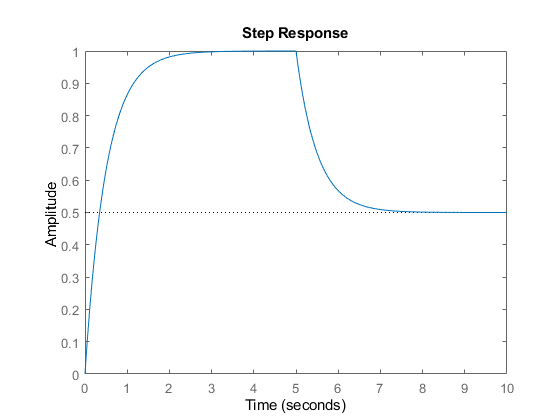
\includegraphics[width=0.8\textwidth]{step.png}}
	    		\end{figure}
		\end{column}
	\end{columns}
\end{frame}

\begin{frame}%[allowframebreaks]
	\frametitle{Model matematyczny statku powietrznego V}
	Oddziaływanie aerodynamiczne:
	\begin{columns}
		\begin{column}{0.4\textwidth}
	   	 	\begin{figure}
	   		 \centering
	      		 \uncover<2->{
	      		 \[
	      		 	\bm{f_A} = \frac{1}{2}\rho V_{T}^2  \bm{S} \bm{C}\left(\alpha, \beta, \bm{x}, \bm{\delta}, ... \right)
			\]}

	    		\end{figure}
		\end{column}
		\begin{column}{0.6\textwidth}
	   	 	\begin{figure}
	   		 \centering
	      		 \uncover<4->{ 
	      		 \[
	      		 	 \bm{C} \approx \bm{C0} + \frac{d\bm{C}}{d\alpha}\alpha + \frac{d\bm{C}}{d\beta}\beta + \frac{d\bm{C}}{d\bm{x}}\bm{x} + \frac{d\bm{C}}{d\bm{\delta}}\bm{\delta}
	      		 \]}
	    		\end{figure}
		\end{column}
	\end{columns}
\end{frame}

\begin{frame}%[allowframebreaks]
	\frametitle{Linearyzacja równań stanu}
	\begin{columns}
		\begin{column}{0.5\textwidth}
				\uncover<2->{\[
						\bm{u} = \begin{bmatrix}\omega_1 \quad \omega_2 \quad ... \quad \omega_n\end{bmatrix}^T
					\]
					\[
						\bm{C} = \bm{I} \hspace{10pt} \bm{D} = \bm{0}
					\]}
				\uncover<3->{\[
				\begin{cases}
					\dot{\bm{x}} \left(t\right)  = \bm{f} \left(t,\bm{x}\left(t\right),\bm{u}\left(t\right) \right) \\
					\bm{y} \left(t\right) = \bm{g} \left(t,\bm{x}\left(t\right),\bm{u}\left(t\right) \right)
				\end{cases}
				\]}	
		\end{column}
		\begin{column}{0.5\textwidth}
	   	 	\uncover<4->{\[
				\begin{cases}
					\dot{\bm{x}} \left(t\right)  = \bm{Ax} \left(t\right)  + \bm{Bu} \left(t\right) \\
					\bm{y} \left(t\right) = \bm{Cx} \left(t\right) + \bm{Du} \left(t\right)
				\end{cases}
				\]}
		\end{column}
	\end{columns}
\end{frame}


\section{Klasyczne metody sterowania wielowirnikowcem}

\begin{frame}
	\frametitle{Sterowanie statkiem powietrznym}
	\begin{figure}
	   		 \centering
	      		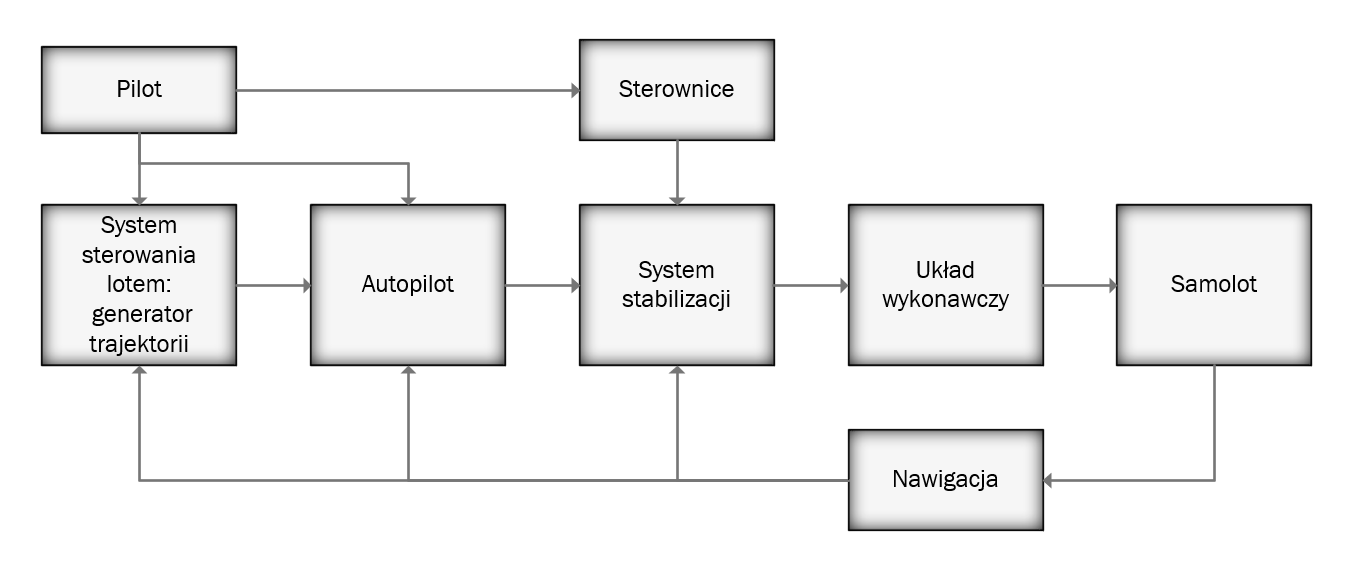
\includegraphics[width=\textwidth]{controller.png}
	\end{figure}
\end{frame}

\begin{frame}
	\frametitle{Sterowanie statkiem powietrznym II}
	\begin{figure}
	   		 \centering
	      		 \includegraphics[width=1.05\textwidth]{pid\_cascade.jpg}
	\end{figure}
\end{frame}


\section{Wykorzystanie regulatora LQR}

\begin{frame}
	\frametitle{Regulator LQR}
	\uncover<2->{
	\[
		Q = \int_{t_0}^{\infty} \left(  \bm{x}^T \bm{Q} \bm{x} + \bm{u}^T \bm{R} \bm{u} \right) dt
	\]}
	\uncover<3->{\[
		\bm{u} = - \bm{K} \bm{x}
	\]}
	\uncover<3->{\[
		\bm{K} = - \bm{R}^{-1} \bm{B}^T \bm{P}
	\]
	\[
		\bm{A}^T \bm{P} + \bm{P}\bm{A} -  \bm{P}\bm{B} \bm{R}^{-1}\bm{B}^T \bm{P} + \bm{Q}
	\]}
\end{frame}

\begin{frame}
	\frametitle{Wizualizacja}
	\href{https://jordan787878.github.io/firstweb/6dofQuadcopter/6dofQuad_LQR.html}{\beamergotobutton{Link}}
\end{frame}

\begin{frame}{Literatura}
\begin{thebibliography}{10}
\beamertemplatebookbibitems
\bibitem{en15197136}[Energies, 2022] Quadrotor Model for Energy Consumption Analysis
   \newblock  Jacewicz, Mariusz and Żugaj, Marcin and Głębocki, Robert and Bibik, Przemysław
 \bibitem{ICIEV}[2013] PID, LQR and LQR-PID on a quadcopter platform.
 \newblock  Argentim, Lucas and Rezende, W.C. and Santos, Paulo and Aguiar, Renato.
  \bibitem{bbb} Quadcopter Control System Design and Implementation with LQR assisted by Kalman Filter: An Experimental Study
\newblock LUDWIG HORVATH and MARTIN PETRÉ
\bibitem{ccc} Design and Development of Optimal Control System (...)
\newblock Zaid Tahir, Mohsin Jamil, Saad Ali Liaqat, Lubva Mubarak, Waleed Tahir and Syed Omer Gilani
\end{thebibliography}
\end{frame}

\begin{frame}
	\frametitle{Dyskusja}
	\begin{figure}
		\centering
		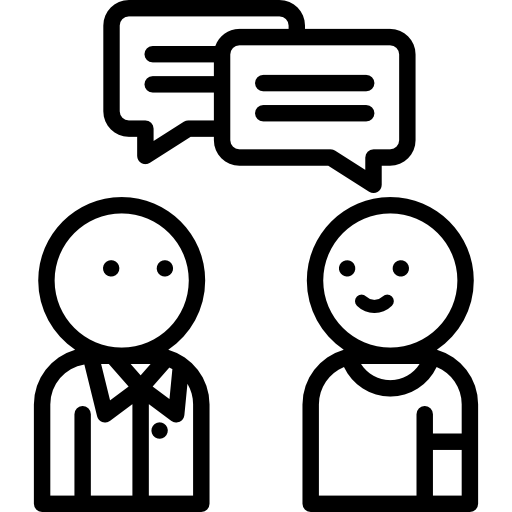
\includegraphics[width=0.7\textwidth]{questions.png}
	\end{figure}
\end{frame}

\begin{frame}
	  \begin{center}
	\Huge Dziękuję za uwagę!
	\end{center}
\end{frame}

\end{document}